\documentclass[12pt,a4paper]{article}

% ─── Packages ─────────────────────────────────────────────────
\usepackage[utf8]{inputenc}
\usepackage[T1]{fontenc}
\usepackage{lmodern}
\usepackage{geometry}
\usepackage{titlesec}
\usepackage{enumitem}
\usepackage{graphicx}
\usepackage{xcolor}
\PassOptionsToPackage{hyphens}{url}
\usepackage{hyperref}
\usepackage{booktabs}
\usepackage{array}
\usepackage{longtable}
\usepackage{parskip}
\usepackage{fancyhdr}
\usepackage{lastpage}
\usepackage[htt]{hyphenat}
\usepackage{microtype}

% Allow typewriter font to break across lines at common punctuation
\makeatletter
\def\UrlBreaks{\do\/\do\-\do\_\do\.\do\=\do\?\do\&\do\#\do\:\do\@}
\makeatother

% Allow LaTeX more flexibility on difficult paragraphs to avoid overfull hboxes
\sloppy
\emergencystretch=3em

% ─── Page geometry ────────────────────────────────────────────
\geometry{margin=2.5cm}
\pagestyle{fancy}
\fancyhf{}
\fancyhead[L]{\small CSC2106 --- Real-Time File Transfer System using CoAP}
\fancyhead[R]{\small BugattiFerrariLamborghini}
\fancyfoot[C]{\thepage\ of \pageref{LastPage}}

% ─── Section formatting ──────────────────────────────────────
\titleformat{\section}{\large\bfseries}{Section \Roman{section}: }{0em}{}
\titleformat{\subsection}{\normalsize\bfseries}{\thesubsection}{1em}{}

% ─── Hyperref ─────────────────────────────────────────────────
\hypersetup{
    colorlinks=true,
    linkcolor=blue,
    citecolor=blue,
    urlcolor=blue
}

% ─── Custom commands ──────────────────────────────────────────
\DeclareRobustCommand{\changed}[1]{\textcolor{red}{#1}}
\DeclareRobustCommand{\forecast}[1]{\textbf{[Forecasted]} #1}

\begin{document}

% ═════════════════════════════════════════════════════════════
% TITLE PAGE
% ═════════════════════════════════════════════════════════════

\begin{center}
    \vspace*{1cm}
    {\Large \textbf{Project: [CSC2106] Real-Time File Transfer System using CoAP}} \\[0.5cm]
    {\large Date: 18 March 2026} \\[0.3cm]
    {\large Group 02: BugattiFerrariLamborghini} \\[1cm]

    \begin{tabular}{|p{7cm}|p{4cm}|}
        \hline
        \textbf{Student Name} & \textbf{Student ID} \\
        \hline
        Pang Jia De & 2402226 \\
        \hline
        Dui Rui En Joshua & 2402201 \\
        \hline
        Tan Jian Xin & 2401421 \\
        \hline
        Tan Bing Kun Terence & 2401883 \\
        \hline
    \end{tabular}

    \vspace{0.8cm}
    \changed{\textbf{Source Code Repository:} \url{https://github.com/Daddycation23/IOTForestCam}}
\end{center}

\vspace{1.5cm}

% ═════════════════════════════════════════════════════════════
% ABSTRACT
% ═════════════════════════════════════════════════════════════

\section*{Abstract}
% (150--250 words)

\changed{Selecting an appropriate communications technology for off-grid forest wildlife monitoring requires balancing range, throughput, and idle power simultaneously. This three-way trade-off cannot be resolved by any single radio stack. This project surveys seven candidate wireless technologies against the constraints of battery-only operation, absence of cellular infrastructure, multi-megabyte image payloads, and multi-hop coordination, then builds and validates a prototype around the only combination that satisfies all five hard constraints.}
The resulting system is a Hybrid IoT Mesh Network built on ESP32-S3 microcontrollers with LILYGO T3-S3 V1.2 boards featuring the SX1280 2.4\,GHz LoRa transceiver. The architecture decouples the control and data planes: LoRa serves as a low-power control plane, while sensor nodes use timer-based deep sleep ($<$10\,$\mu$A) with 180-second wake intervals. \changed{The gateway runs a persistent Wi-Fi access point. Leaf nodes connect as station clients on timer wake and serve images for download via CoAP.} Image payloads are segmented and \changed{reliably} transmitted \changed{over the Wi-Fi data plane} using CoAP block-wise transfer over UDP. \changed{AODV reactive mesh routing enables multi-hop coordination, and a Bully election algorithm provides automatic gateway selection.} By shifting from a continuous-listening network to an event-driven hybrid model, this system minimizes idle power consumption while retaining the capacity to route large files across multiple hops. The prototype demonstrates a potentially scalable, energy-efficient framework capable of delivering visual alerts to a local gateway, shifting remote forest monitoring from reactive manual data retrieval to proactive intervention.

\newpage

% ═════════════════════════════════════════════════════════════
% SECTION I: INTRODUCTION, PROBLEM STATEMENT AND OBJECTIVES
% ═════════════════════════════════════════════════════════════

\section{Introduction, Problem Statement and Objectives}
% (Word Limit: 750 words)

\subsection{Introduction}

Effective environmental monitoring and forest conservation is critical for biodiversity preservation and disaster mitigation, which require sensor networks capable of operating autonomously in remote, off-grid environments. Currently, the industry relies on manual data retrieval from local storage, which is labor-intensive and reactive. This project proposes a Hybrid IoT Mesh Network utilizing ESP32-S3 microcontrollers to bridge the gap between remote sensing and real-time data access. By integrating LoRa for long-range, low-power control signaling and Wi-Fi for high-bandwidth data transfer, the system offers a scalable solution. \changed{To ensure rigorous and deterministic validation of the underlying network routing, this iteration of the project replaces live camera hardware with an SD card containing pre-loaded images. This approach utilizes images with various resolutions pre-loaded onto SD cards, eliminating camera hardware-induced errors and isolating the network's performance metrics for more accurate testing.} The system employs periodic wake cycles combined with event-driven coordination, enabling all high-bandwidth communications to utilize CoAP over UDP for lightweight, reliable image transmission via block-wise transfer. This architecture shifts remote monitoring from reactive data retrieval to proactive intervention.

\subsection{Problem Statement}

The primary challenge in off-grid environmental monitoring is the ``Data Latency Gap.'' Standard methods store data locally on SD cards, resulting in weeks or months of delay between an event occurring and its detection. While real-time wireless alternatives exist, they face a strict ``Bandwidth-Range-Power Trilemma'': low-power wide-area technologies (like LoRa) lack the bandwidth required for image transfer, while high-bandwidth solutions (like standard Wi-Fi or cellular networks) consume excessive energy and lack coverage in deep forests.

This project directly addresses this gap by decoupling the control and data transport layers, solving the power constraints that traditionally limit the long-term deployment of visual sensors. \changed{Furthermore, traditional embedded vision nodes frequently suffer from heap memory exhaustion when processing large image buffers in real-time. By implementing a storage-driven data pipeline that streams data directly from an SD card to the Wi-Fi buffer in 1024-byte chunks, this project circumvents the 512\,kB SRAM limit of the ESP32-S3 [1]. Additionally, the network design has been improved to operate completely independently of commercial LoRaWAN or 4G infrastructure; the gateway is now implemented purely as a designated ``Root Node'' within the network, bridging directly to a local diagnostic server for localized, off-grid deployment.}

\subsection{Objectives}

The main goal of this project is to develop and validate a functional prototype of a hybrid sensor node that overcomes the limitations of single-protocol networks. The specific objectives are categorized into implemented features and future work:

\subsubsection{Implemented Objectives}

\begin{enumerate}
    \item \textbf{Design a Hybrid Network Architecture:} Develop a sensor node utilizing the ESP32-S3 that integrates both LoRa \changed{(SX1280)} and Wi-Fi radios to optimize the trade-off between transmission range and data bandwidth.

    \item \textbf{Implement Low-Power Sleep Management:} Engineer an efficient power management system using timer-based deep sleep ($<$10\,$\mu$A) with 180-second wake intervals. \changed{Note: The originally planned LoRa DIO1 hardware interrupt wake mechanism is non-functional on the LILYGO T3-S3 V1.2 hardware; timer-based wake serves as the primary implementation.}

    \item \textbf{Optimize Image Transfer:} Implement CoAP over UDP with Block-Wise Transfer mechanisms to enable the reliable transmission of large payloads over a lossy, multi-hop Wi-Fi mesh.

    \item \textbf{Develop Dynamic Role Assignment:} Implement a flexible role configuration system allowing all ESP32-S3 nodes to be assigned as Leaf, Relay, or Gateway at deployment, with persistence across power cycles. \changed{Extend this with automatic role negotiation via a Bully election algorithm, enabling nodes to self-organize without manual configuration.}

    \item \changed{\textbf{Develop a File Reading Pipeline:} Design an SD-card-based file I/O system that simulates physical camera captures by randomly reading and segmenting pre-loaded JPEG files into network-safe chunks, ensuring stable payload generation without memory allocation failures.}

    \item \textbf{Evaluate System Performance:} Quantitatively assess the prototype against standard engineering metrics, specifically measuring idle power consumption, total network throughput, and successful multi-hop packet delivery rates in a simulated deployment environment.
\end{enumerate}

\subsubsection{Future Work}

The following objectives remain as planned enhancements beyond the current implementation scope:

\begin{enumerate}
    \item \textbf{Implement Queue-Based Scheduling:} Design a gateway-managed transmission queue that assigns time-division slots to prevent network congestion, ensuring only one node transmits image data at a time. \changed{Current implementation uses sequential harvest without explicit time-slot allocation.}

    \item \textbf{Security and Encryption:} Implement AES-128 encryption for LoRa control-plane packets to protect against eavesdropping and tampering. \changed{Current implementation transmits all packets in cleartext.}
\end{enumerate}

\newpage

% ═════════════════════════════════════════════════════════════
% SECTION II: LITERATURE REVIEW
% ═════════════════════════════════════════════════════════════

\section{Literature Review}
\label{sec:lit-review}

Environmental monitoring is transitioning from manual data collection to connected Wireless Sensor Networks [2], but deployments remain fragmented. High-bandwidth networks (4G/LTE, Wi-Fi) lack coverage in remote forests and require substantial power infrastructure [3]. LPWANs like LoRa provide multi-kilometer range with idle current $<$20\,$\mu$A but are limited to 222-byte payloads and throughput $<$5\,kbps [4]. No single wireless technology simultaneously provides long range, high throughput, low idle power, and licence-free operation.

The radio stack selection is constrained by five hard requirements: (H1) battery-only operation with average current $<$100\,$\mu$A on a 2000\,mAh LiPo; (H2) no cellular or upstream network access; (H3) image payloads of at least 50\,kB must traverse the network within a single harvest cycle at effective goodput above 10\,kB/s; (H4) multi-hop coordination without pre-configured routing; (H5) operation on commodity ESP32-S3 hardware. Three soft preferences apply: low cost, mature open-source firmware, and team familiarity.

Mapping candidates to these requirements yields clear rejections. LoRaWAN fails H3 and H4. Wi-Fi fails H1. BLE fails the range constraint. Zigbee fails H3 and H5. LTE-M and NB-IoT fail H2. Sigfox fails H3. The LoRa 2.4\,GHz + Wi-Fi hybrid satisfies them jointly: LoRa carries control-plane traffic at sub-20\,$\mu$A idle and kilometre-scale range, while Wi-Fi carries bulk image payloads at 10+\,Mbps with idle power amortised across deep-sleep intervals. This dual-plane decomposition is the central design decision, justified in Section~\ref{sec:design}.

Energy-consumption modelling studies show LoRa battery lifetimes of months to years are achievable [5]. Where [5] establishes energy viability for sensing, [6] demonstrates that reactive routing can operate within this budget through on-demand path discovery. Hybrid-network literature corroborates that neither approach alone suffices: single-radio systems cannot handle long-range idle listening and high-speed data bursts simultaneously. Hybrid LoRa-plus-Wi-Fi approaches corroborate this, trading Wi-Fi's idle power for bursty throughput while LoRa maintains always-on control-plane coverage.

Commonly used methodologies involve single-radio duty-cycling, where a high-bandwidth node wakes on a fixed schedule. \changed{This is ineffective for real-time alerts because the network is ``deaf'' between cycles.} Another methodology transmits compressed images exclusively over LoRa. An experimental study of small JPEG image transmission over LoRa reports on-air times of under two minutes at SF7 rising to roughly 14 minutes at SF12, with a delivery success rate of only about 57\% [7]. This is ineffective for bulk transfer and depletes batteries rapidly.

The primary limitation of existing solutions is the ``Bandwidth-Range-Power Trilemma.'' High-bandwidth radios consume 80--200\,mA idle, draining a 2000\,mAh battery in 10--25 hours. Low-power radios operate at $<$20\,$\mu$A idle but cannot handle media files. Furthermore, existing embedded vision methodologies overlook memory constraints: the ESP32-S3 provides 512\,kB SRAM [1], but typical JPEG images range from 50--200\,kB, and instruction memory, network stacks, and application state consume the remainder. Loading entire image buffers into RAM causes heap exhaustion.

These findings inform this study's design. Decoupling control and data planes across LoRa and Wi-Fi (Objective \#1) targets the trilemma. Timer-based deep sleep with 180-second wake intervals (Objective \#2) bounds latency while preserving $<$10\,$\mu$A idle current. LoRa image transfer success rates below 60\% in [7] inform using LoRa exclusively for control packets $<$100 bytes (Objective \#3). The SRAM budget [1] drives the storage-driven pipeline design (Objective \#5): streaming 1024-byte chunks via CoAP block-wise transfer (RFC 7959 [8]) eliminates heap exhaustion.

\newpage

% ═════════════════════════════════════════════════════════════
% SECTION III: DESIGN
% ═════════════════════════════════════════════════════════════

\section{Design}
\label{sec:design}

\subsection{Overall System Architecture}

\changed{The selection of LoRa 2.4\,GHz (SX1280) for the control plane and ESP32 Wi-Fi for the data plane follows directly from the technology comparison in Section~\ref{sec:lit-review}.} Building on this dual-plane decomposition, the physical topology organises as shown in Figure~\ref{fig:arch}.

\begin{figure}[ht]
\centering
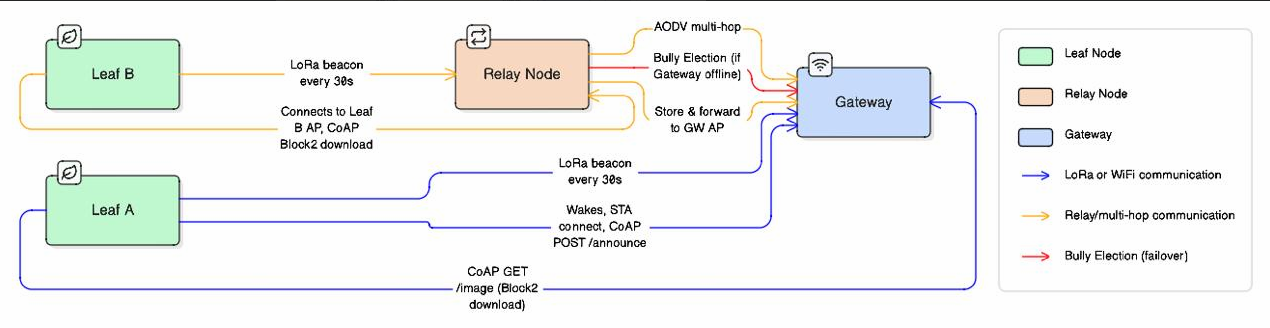
\includegraphics[width=0.9\linewidth]{../docs/figures/High-Level-Architecture.png}
\caption{High-level architecture of the hybrid LoRa + Wi-Fi mesh. LoRa 2.4\,GHz forms the control-plane mesh (beacons, AODV routing, Bully election, harvest coordination). Wi-Fi forms the data-plane star via the gateway's persistent access point, with leaves connecting as STA clients for CoAP Block-Wise image transfer. Out-of-range leaves are serviced by a relay node performing sequential store-and-forward.}
\label{fig:arch}
\end{figure}

\begin{itemize}
    \item \textbf{Control Plane (LoRa: Mesh topology):} All nodes broadcast beacons and routing packets over LoRa 2.4~GHz. AODV reactive routing discovers multi-hop paths, and a Bully election algorithm selects the gateway.
    \item \textbf{Data Plane (Wi-Fi: Star topology):} The gateway runs a persistent Wi-Fi access point. Leaf nodes connect as station (STA) clients to transfer images via CoAP. For out-of-range leaves, a relay node performs sequential store-and-forward between the leaf's AP and the gateway's AP.
\end{itemize}

\subsection{Hardware and Devices}

The network is composed of identical hardware nodes acting in different roles (Leaf, Relay, and Gateway). Each node utilizes:

\begin{enumerate}
    \item \textbf{Microcontroller:} Espressif ESP32-S3 [1] (managing logic and Wi-Fi).
    \item \textbf{Transceiver:} \changed{SX1280 2.4\,GHz LoRa module [9] on the LILYGO T3-S3 V1.2 board (handling the control plane).}
    \item \textbf{Display:} SSD1306 128$\times$64 OLED via I2C for real-time status.
    \item \textbf{File Transfer:} A MicroSD Card module via HSPI. Pre-loaded JPEG images on the SD card simulate physical camera captures.
\end{enumerate}

\subsection{Network Topology and Connections}

\changed{The current prototype uses AODV reactive routing over the LoRa control plane for multi-hop coordination. The gateway runs a persistent Wi-Fi AP. Leaf nodes wake from deep sleep on a 180-second timer, connect as STA clients to the gateway's AP, and send a CoAP POST /announce message. The gateway then downloads images from the leaf's STA IP via CoAP Block2 pipelined transfer.} For multi-hop nodes (out of direct Wi-Fi range), a relay node performs sequential store-and-forward: connecting first to the leaf's AP, caching images locally, then connecting to the gateway's AP to deliver them.

\subsection{Data Collection and Communication Protocols}

Data collection is driven by a storage-to-network pipeline: the ESP32-S3 reads pre-loaded JPEGs from the SD card in 1024-byte chunks, avoiding loading entire files into RAM. This chunk size maps directly onto the communication protocol stack, which comprises three layers:

\begin{enumerate}
    \item \textbf{Control Protocol:} \changed{LoRa 2.4\,GHz physical layer is used for beacon discovery, AODV routing (RREQ/RREP/RERR), election packets, and harvest commands.}
    \item \textbf{Transport Protocol:} Data routing over Wi-Fi relies on CoAP (Constrained Application Protocol) over UDP [10].
    \item \textbf{Data Transfer Mechanism:} CoAP Block-Wise Transfer [8] maps 1024-byte SD card chunks to CoAP block sizes, fitting within the 1500-byte Wi-Fi MTU to prevent IP fragmentation. \changed{Pipelined requests with a window of 3 and 2-second timeout improve throughput.}
\end{enumerate}

\subsection{Data Storage and Processing}

Data storage is decentralized at the edge. Raw data (simulated images) resides on the local SD cards of individual leaf nodes. Harvesting is a copy operation: the gateway saves harvested images with unique filenames incorporating node MAC suffix, boot count, and uptime. Computational tasks such as image reconstruction or full-file buffering are avoided on the constrained microcontrollers.

\subsection{User Interaction and Integration}

As this system is designed for remote, off-grid environmental monitoring, it avoids integration with third-party cloud platforms. Users interact through four local mechanisms:

\begin{enumerate}
    \item \textbf{Local SD Card Access:} The gateway saves harvested images to its local SD card \texttt{/received/} directory. Users retrieve images via physical SD card removal or USB serial file transfer.
    \item \textbf{Serial Command Interface:} Runtime management via serial commands (\texttt{block}, \texttt{unblock}, \texttt{list}) allows dynamic control of which nodes participate in harvest cycles.
    \item \textbf{OLED Status Display:} Each node displays real-time status (role, IP address, image count, network statistics) for rapid field diagnosis.
    \item \changed{\textbf{Python Host-Side Tools:} Terminal and GUI dashboards parse serial statistics for live monitoring, and a standalone image downloader supports CoAP pull and SD browse modes.}
\end{enumerate}

\subsection{Security Protocols}

The gateway's Wi-Fi access point uses WPA2-PSK encryption with a static pre-shared key, preventing unauthorized devices from joining the network. LoRa control packets include a 3-byte magic header (\texttt{0xFC 0x01 type}) to distinguish ForestCam traffic from environmental noise, adequate for laboratory testing but not providing cryptographic authentication. AES-128 encryption for LoRa packets and HMAC-SHA256 mutual authentication are planned for field deployment.

\newpage

% ═════════════════════════════════════════════════════════════
% SECTION IV: IMPLEMENTATION (PROTOTYPE AND TESTING)
% ═════════════════════════════════════════════════════════════

\section{Implementation (Prototype and Testing)}
% (Word Limit: 750 words)

\textit{Note: The final implementation differs from the originally proposed design in several areas:}

\begin{itemize}
    \item \textit{\textbf{Mesh Routing:} ESP-Mesh-Lite was replaced with AODV-over-LoRa routing. ESP-Mesh-Lite requires all nodes to remain continuously awake, which is fundamentally incompatible with the deep-sleep power management required for sub-100\,$\mu$A average current.}
    \item \textit{\textbf{Power Management:} LoRa DIO1 hardware interrupt wake was replaced with RTC timer-based wake (180-second intervals). The SX1280 loses receive capability during ESP32-S3 deep sleep because RXEN/TXEN GPIO holds are insufficient to maintain the PA control lines on the LILYGO T3-S3 V1.2.}
    \item \textit{\textbf{Gateway Architecture:} The gateway now runs a persistent Wi-Fi AP instead of sequentially connecting to individual leaf APs. This eliminates Wi-Fi hopping overhead, enables simultaneous leaf connections, and aligns with the timer-based wake approach.}
\end{itemize}

\textit{Host-side Python tools (\texttt{dashboard.py}, \texttt{dashboard\_gui.py}, \texttt{viewer.py}, \texttt{flash\_and\_monitor.py}) support live monitoring, CoAP image retrieval, and parallel flash/monitor operations.}

\subsection{Prototyping and Development Tools}

The system is prototyped using LILYGO T3-S3 V1.2 development boards integrating the ESP32-S3 and SX1280 2.4\,GHz LoRa. Development is conducted in C++ using PlatformIO (Visual Studio Code). The software stack relies on RadioLib for SX1280 interrupt handling, custom C++ implementations for CoAP (RFC 7252/7959), AODV routing (RFC 3561), Bully election, and deep sleep management. FreeRTOS (built into ESP-IDF) provides dual-core task scheduling.

\subsection{Deployment Strategy, Challenges, and Mitigation}

The prototype is deployed in a laboratory environment for bench-testing. Key challenges and mitigations include:

\begin{enumerate}
    \item \textbf{SPI Bus Conflicts:} \changed{Resolved by placing LoRa and SD card on separate hardware SPI buses (FSPI for LoRa, HSPI for SD) on the LILYGO T3-S3 board.}

    \item \textbf{High Packet Loss on UDP:} CoAP runs over UDP, so dropped packets are not automatically resent. Mitigation: the application layer requires explicit ACKs for every 1024-byte block with retransmission on timeout. \changed{Pipelined download includes a per-image retry mechanism.}

    \item \changed{\textbf{LoRa Blackout During Harvest:} FreeRTOS dual-core task separation pins LoRa/AODV/election to Core 0 and Wi-Fi/CoAP harvest to Core 1, allowing concurrent operation.}

    \item \changed{\textbf{LoRa/Wi-Fi Range Mismatch:} The SX1280 has longer range than the ESP32-S3 Wi-Fi. Mitigation: Wi-Fi transmit power is raised to 19.5\,dBm, and a WiFi-fail relay fallback issues a \texttt{HARVEST\_CMD} over LoRa when direct connection times out.}

    \item \textbf{Environmental Signal Attenuation:} Dense foliage absorbs 2.4\,GHz Wi-Fi signals, potentially fragmenting the data plane. Mitigation: AODV reactive routing discovers alternative paths through relay nodes; unreachable nodes trigger RERR packets that re-initiate route discovery.

    \item \textbf{SoftAP Concurrent STA Limit:} The ESP32-S3 SoftAP supports approximately 4 simultaneous STA connections. Mitigation: the 180-second timer wake with MAC-based jitter staggers leaf connections, reducing the probability of association contention.
\end{enumerate}

\subsection{Testing Process for Reliability and Functionality}

Testing progresses from unit tests to system integration:

\begin{enumerate}
    \item \textbf{Unit Testing:} \changed{181 unit tests across 19 test suites cover election state machines, harvest FSM transitions, CoAP Block2 pipelining, beacon serialization, AODV route expiry, and thread safety.}

    \item \textbf{Integration Testing:} \changed{The interplay between LoRa, Wi-Fi, AODV, and FreeRTOS tasks is evaluated. Thread-safety of shared variables (\texttt{std::atomic}) was validated through code review and runtime testing.}

    \item \textbf{System-Level Testing:} A 3-node topology (Gateway, Relay, Leaf) is deployed in laboratory conditions. \changed{Auto-role negotiation allows testing without manual role assignment. Image transfer is validated over both direct Wi-Fi and relay store-and-forward paths.}
\end{enumerate}

\changed{Testing to date covers unit-level verification (all 181 tests passing) and two system-level deployments: a 3-node laboratory bench and a 3-node corridor field test with bidirectional LoRa MAC blocks forcing a 2-hop relay path. The following test activities are deferred and tracked in \texttt{ref/PENDING\_MEASUREMENTS.md}:}

\begin{enumerate}
    \item \textbf{Security Testing:} Penetration testing, LoRa replay attack validation, and WPA2-PSK key strength audits.
    \item \textbf{Quantitative Power Measurement:} Multimeter measurement of deep-sleep idle current and active harvest current.
    \item \textbf{Multi-Hop Stress Testing:} Chains beyond 2 hops and concurrent relay operations.
    \item \textbf{Scalability Testing:} 4-to-8-node deployments and SoftAP concurrent STA saturation tests.
    \item \textbf{Outdoor Environmental Testing:} Longer deployments with foliage attenuation, temperature extremes, and wet-weather interference.
\end{enumerate}

\subsection{Evaluation Metrics and Benchmarks}

\changed{The following evaluation criteria have been recorded:}

\begin{enumerate}
    \item \textbf{Data Integrity:} Fletcher-16 checksums computed on the leaf and verified at the gateway through a dedicated \texttt{/checksum} CoAP endpoint.

    \item \textbf{Functional Image Delivery:} CoAP Block-Wise Transfer delivers complete JPEG images (50\,kB to 5\,MB) over both direct Wi-Fi and relay store-and-forward paths.

    \item \textbf{Auto-Role Negotiation:} Bully election promotes the highest-priority node within a 15-second startup grace period.

    \item \textbf{Packet Counters:} Per-boot counters track LoRa TX/RX/errors, AODV RREQ/RREP/RERR, beacon TX/RX, and harvest totals, emitted as a \texttt{[STATS]} serial line every 5\,s.

    \item \changed{\textbf{First Measurement Run (2026-04-05, 4-node lab, 300\,s):} Beacon broadcast PDR 100\%, LoRa all-layer PDR 74.51\%, CoAP Block2 goodput mean 10.29\,KB/s, Bully election convergence 25.9\,s, beacon-reactive harvest trigger 15.16\,s, Fletcher-16 mismatch rate 0/42. Detailed results are in Section~V.}
\end{enumerate}

\newpage

% ═════════════════════════════════════════════════════════════
% SECTION V: RESULTS AND ANALYSIS
% ═════════════════════════════════════════════════════════════


\section{Results and Analysis}

\subsection{Implementation Status}

The dual-radio architecture using \changed{SX1280 2.4\,GHz LoRa} for the control plane and ESP32-S3 Wi-Fi for the data plane is fully operational, as verified by 181 passing unit tests, a 3-node laboratory deployment, and a 3-node corridor field test. CoAP Block-Wise Transfer (RFC 7959) with 1024-byte blocks and pipelined requests (window of 3, 2-second timeout) delivers complete JPEG images (50\,kB to 5\,MB) with zero Fletcher-16 checksum mismatches across 42 transfers. AODV reactive routing with a 12-entry route table and 120-second expiry replaced the originally proposed ESP-Mesh-Lite approach. Auto-role negotiation via Bully election with a 15-second grace period, timer-based deep sleep at 180-second intervals, relay store-and-forward, and Fletcher-16 checksum verification are all operational. FreeRTOS dual-core task separation eliminated 50--120\,s LoRa blackouts during harvest. The gateway-as-AP architecture replaced sequential Wi-Fi hopping, and beacon-reactive harvest reduced trigger latency from 180\,s fixed cycles to under 15\,s.

AES-128 LoRa encryption, queue-based TDMA scheduling, and leaf-side WiFi-fail relay fallback remain future work.

\subsection{Key Performance Metrics}

\changed{A 4-node laboratory capture (300\,s window) produced the following quantitative results:}

\begin{itemize}
    \item \textbf{Data Integrity:} \changed{Fletcher-16 mismatch rate 0.00\% (42 PASS / 0 FAIL) across direct and relayed CoAP paths.}
    \item \changed{\textbf{CoAP Block2 Goodput:} Mean 10.29\,KB/s, median 9.90\,KB/s, range 7.00--14.90\,KB/s over N=21 single-hop transfers.}
    \item \changed{\textbf{Packet Delivery:} Beacon broadcast PDR 100\% (N=108 expected), LoRa all-layer PDR 74.51\% (aggregated across beacons, AODV, and election packets).}
    \item \changed{\textbf{Control-Plane Latency:} Bully election convergence 25.9\,s, beacon-reactive harvest trigger 15.16\,s.}
\end{itemize}

Multi-hop routing was validated qualitatively in a 3-node corridor field test (Feature 26) using bidirectional LoRa MAC blocks to force a 2-hop relay path, confirming AODV route formation and successful image harvest through the relay.

\changed{Scalability is constrained by firmware limits: the NodeRegistry holds 8 nodes, the AODV route table holds 12 entries, and the SoftAP accepts roughly 4 concurrent STA clients. The 74.51\% LoRa all-layer PDR at 4 nodes may indicate channel congestion in a packed half-duplex topology, though RF interference or packet collisions could also contribute. Exceeding the SoftAP limit causes association rejections that the 180-second timer with MAC-based jitter helps mitigate.}

\subsection{Effectiveness of the Selected Communications Technology}
\label{sec:effectiveness}

\changed{The core claim tested is that a LoRa 2.4\,GHz plus Wi-Fi hybrid solves the bandwidth-range-power trilemma that no single candidate technology can satisfy alone. The recorded evidence is as follows.}

\changed{\textbf{LoRa 2.4\,GHz control plane:} Beacon discovery, AODV routing, Bully election, and harvest coordination operate over LoRa using a 15-byte v2 beacon format every 30\,s. In the corridor test, bidirectional MAC blocks forced the gateway and leaf onto opposite sides of a relay: AODV formed a 2-hop path, and the gateway harvested images through the relay. This confirms LoRa 2.4\,GHz suffices for the control plane over multi-hop topologies.}

\changed{\textbf{Wi-Fi data plane:} CoAP Block2 transfer at 1024-byte blocks delivered N=21 JPEG images at mean 10.29\,KB/s with zero Fletcher-16 mismatches across 42 checksums. The resume-offset mechanism persists progress to RTC memory, so interrupted transfers resume from the last completed block.}

\changed{\textbf{Trilemma resolution:} The hybrid satisfies the hard constraints jointly: LoRa provides the low idle current and multi-hop range that Wi-Fi alone cannot, while Wi-Fi provides the multi-megabyte throughput that LoRa alone cannot, and both radios share the commodity LILYGO T3-S3 board. The architectural cost is the loss of instantaneous cross-radio wake: the SX1280 DIO1 line cannot reliably wake the ESP32-S3 from deep sleep on this board, so the system uses timer-based wake at 180\,s intervals. This trades sub-second alerting for bounded periodic harvest latency.}

\changed{\textbf{Comparison with pure-LoRa image transfer:} Prior work [7] reports that delivering a small JPEG image over LoRa requires on-air times of under two minutes at SF7 rising to roughly 14 minutes at SF12, with a delivery success rate of only about 57\%. This project carries all image bytes over Wi-Fi at Mbps-class throughput, so per-image time is limited by Wi-Fi setup and CoAP turnaround rather than radio airtime, and the LoRa channel remains free for routing traffic.}

\subsection{Bottlenecks and Challenges}

\changed{The primary bottleneck is the ESP32 SoftAP limit of approximately 4 concurrent STA connections. Leaves that wake simultaneously compete for association slots, and sequential CoAP downloads add per-node transfer latency proportional to image count and size.}

\changed{\textbf{FreeRTOS Thread Safety:} Shared variables accessed from both cores were changed to \texttt{std::atomic} to prevent data races, and a spinlock was added around the relay ACK struct copy.}

\changed{\textbf{Multi-Gateway Election Race:} During 3-node hardware testing, all nodes self-promoted to gateway simultaneously. Root causes: LEAF nodes did not process received beacons for gateway detection, promoted nodes beaconed with the wrong role, and a fixed grace period created a race on the half-duplex channel. Fixes: moved beacon processing outside the RELAY-only gate, corrected role in beacons, and added MAC-based jitter to stagger grace periods.}

\changed{\textbf{Security Effectiveness:} WPA2-PSK on the gateway AP provides baseline security that appears adequate for laboratory testing. The LoRa magic header distinguishes ForestCam traffic from environmental noise but does not provide cryptographic security. All LoRa control packets remain in cleartext, leaving the system theoretically vulnerable to replay attacks in uncontrolled environments.}

\changed{\textbf{SPI Bus Resolution:} The SPI bus conflict between the SX1280 LoRa module and the SD card was resolved by placing them on separate hardware SPI buses (FSPI for LoRa, HSPI for SD) on the LILYGO T3-S3 board.}

\changed{\textbf{Memory Management:} The 1024-byte chunked reading approach from the storage pipeline prevents heap exhaustion. No memory allocation failures have been observed during sustained multi-image transfers.}

\changed{\textbf{Implementation Bugs Found and Fixed:} A buffer overflow in \texttt{CoapClient::verifyChecksum()} was discovered during code review: writing a null byte at \texttt{buf[128]} when the buffer was 128 bytes. This was fixed by allocating 129 bytes and limiting the read to 128. A blocking \texttt{delay()} call was replaced with \texttt{vTaskDelay()} to prevent FreeRTOS scheduler starvation.}

\changed{All six original objectives are either fully implemented or explicitly deferred as future work (AES-128 encryption, TDMA scheduling).}



\section{Conclusion}

\changed{The central finding of this project is that the off-grid forest wildlife monitoring problem cannot be solved by any single communications technology among the seven candidates surveyed. A structured comparison against five hard constraints leaves only the LoRa 2.4\,GHz plus Wi-Fi hybrid as a viable candidate, and the prototype validates this selection.}
The prototype decouples low-power control signalling (LoRa SX1280) from high-bandwidth data transfer (ESP32 Wi-Fi) on commodity ESP32-S3 hardware. CoAP Block-Wise Transfer (1024-byte blocks) over Wi-Fi, combined with AODV multi-hop routing over LoRa, reliably transfers JPEG images (50\,kB to 5\,MB) across a 3-node laboratory topology and a 3-node corridor field test with Fletcher-16 checksum verification passing end-to-end. The system achieves auto-role negotiation via Bully election, timer-based deep sleep with 180-second wake intervals, relay store-and-forward, and beacon-reactive harvest reducing trigger latency from 180\,s to under 15\,s.

Future work includes security hardening (AES-128 LoRa encryption, HMAC authentication, WPA2-PSK penetration testing), quantitative measurement runs (deep-sleep current, 2-hop CoAP goodput, scalability beyond 4 nodes, AODV RREQ-to-RREP latency), outdoor field deployment, leaf-side WiFi-fail relay fallback, and TDMA scheduling. \changed{The LoRa DIO1 hardware wake incompatibility on the LILYGO T3-S3 V1.2 is a permanent board-level limitation; timer-based wake with leaf-initiated \texttt{POST /announce} is the selected workaround.}

The prototype suggests that commodity ESP32 hardware is capable of multi-hop file transfer in infrastructure-less environments, pending further validation. This contributes a validated reference architecture for off-grid environmental monitoring that can serve as a foundation for scalable deployments with added security and TDMA scheduling. Transitioning to production deployment requires the measurement and hardening work outlined above.

\newpage

% ═════════════════════════════════════════════════════════════
% AI USAGE ACKNOWLEDGMENT
% ═════════════════════════════════════════════════════════════

\section*{AI Usage Acknowledgment}
\addcontentsline{toc}{section}{AI Usage Acknowledgment}

In line with Singapore Institute of Technology guidelines on the responsible
use of generative artificial intelligence in academic work, the team
acknowledges that Claude (Anthropic's large language model) was used during
the development of this project as a coding, debugging, and documentation
aid. Specific uses included:

\begin{itemize}[leftmargin=1.5em, itemsep=0.2em]
    \item Assistance with implementing the RSSI-based relay assignment,
          ghost-relay demotion logic, packet statistics instrumentation,
          and the self-beacon filter in the firmware.
    \item Debugging guidance during physical corridor tests, including
          interpretation of serial logs, diagnosis of CoAP block-wise
          transfer issues, and analysis of Wi-Fi connection failures.
    \item Development of supporting Python tooling (\texttt{dashboard.py},
          \texttt{packet\_loss\_analyzer.py}, \texttt{measure\_report.py})
          used to capture measurements and generate the quantitative
          results presented in Section V.
    \item Editorial feedback on report structure and phrasing.
\end{itemize}

All AI-generated code, suggestions, and text were reviewed, tested, and
validated by the team before inclusion in the final deliverable. The
architectural decisions, experimental observations, and analysis of results
remain the intellectual work of the team. The following citation is
provided per the APA 7th edition style recommended by the APA blog:

\vspace{0.5em}
\noindent
\hangindent=1.5em
Anthropic. (2026). \textit{Claude} (Opus 4.6 version) [Large language model]. \url{https://claude.ai}

\newpage

% ═════════════════════════════════════════════════════════════
% SECTION VII: REFERENCES
% ═════════════════════════════════════════════════════════════

\section*{References}
\addcontentsline{toc}{section}{References}

\begin{enumerate}[label={[\arabic*]}]
    \item \changed{Espressif Systems, ``ESP32-S3 Series Datasheet,'' Rev. 2.2, 2024. [Online]. Available: \url{https://www.espressif.com/sites/default/files/documentation/esp32-s3_datasheet_en.pdf}}

    \item D. Kandris, C. Nakas, D. Vomvas, and G. Koulouras, ``Applications of Wireless Sensor Networks: An Up-to-Date Survey,'' \textit{Applied System Innovation}, vol. 3, no. 1, art. 14, 2020, doi: 10.3390/asi3010014. [Online]. Available: \url{https://doi.org/10.3390/asi3010014}

    \item \changed{S. N. Jafari and B. M. C. Silva, ``A Survey on Real-Time Data Transfer and Energy Consumption Strategies for Rural and Remote IoT Technologies,'' \textit{IEEE Open Journal of the Computer Society}, vol. 6, pp. 1686--1702, 2025, doi: 10.1109/OJCS.2025.3619210. [Online]. Available: \url{https://doi.org/10.1109/OJCS.2025.3619210}}

    \item F. Adelantado, X. Vilajosana, P. Tuset-Peiro, B. Martinez, J. Melia-Segui, and T. Watteyne, ``Understanding the limits of LoRaWAN,'' \textit{IEEE Communications Magazine}, vol. 55, no. 9, pp. 34--40, 2017, doi: 10.1109/MCOM.2017.1600613. [Online]. Available: \url{https://doi.org/10.1109/MCOM.2017.1600613}

    \item T. Bouguera, J.-F. Diouris, J.-J. Chaillout, R. Jaouadi, and G. Andrieux, ``Energy consumption model for sensor nodes based on LoRa and LoRaWAN,'' \textit{Sensors}, vol. 18, no. 7, art. 2104, 2018, doi: 10.3390/s18072104. [Online]. Available: \url{https://doi.org/10.3390/s18072104}

    \item C. Perkins, E. Belding-Royer, and S. Das, ``Ad hoc On-Demand Distance Vector (AODV) Routing,'' RFC 3561, IETF, Jul. 2003. [Online]. Available: \url{https://www.rfc-editor.org/rfc/rfc3561}

    \item A. H. Jebril, A. Sali, A. Ismail, and M. F. A. Rasid, ``Overcoming Limitations of LoRa Physical Layer in Image Transmission,'' \textit{Sensors}, vol. 18, no. 10, art. 3257, 2018, doi: 10.3390/s18103257. [Online]. Available: \url{https://doi.org/10.3390/s18103257}

    \item \changed{C. Bormann and Z. Shelby, ``Block-Wise Transfers in the Constrained Application Protocol (CoAP),'' RFC 7959, IETF, Aug. 2016. [Online]. Available: \url{https://www.rfc-editor.org/rfc/rfc7959}}

    \item \changed{Semtech Corporation, ``SX1280/SX1281 Long Range, Low Power, 2.4 GHz Transceiver Datasheet,'' Rev. 3.2, Mar. 2020. [Online]. Available: \url{https://www.semtech.com/products/wireless-rf/lora-connect/sx1280}}

    \item \changed{Z. Shelby, K. Hartke, and C. Bormann, ``The Constrained Application Protocol (CoAP),'' RFC 7252, IETF, Jun. 2014. [Online]. Available: \url{https://www.rfc-editor.org/rfc/rfc7252}}
\end{enumerate}

\end{document}